\documentclass[12pt, a4paper, lithuanian]{article}
\usepackage[utf8x]{inputenc}
\def\LTfontencoding{L7x}
\PrerenderUnicode{ąčęėįšųūž}
\usepackage[\LTfontencoding]{fontenc}
\usepackage[lithuanian]{babel}
\usepackage{VUMIFPSkursinis}
\usepackage{cite}
\usepackage{amsmath}
\usepackage{bm}
\usepackage{amsfonts}
\usepackage{float}
\usepackage{graphicx}
\usepackage{color}
\usepackage{listings}
\usepackage{wrapfig}
\usepackage{algpseudocode}
\usepackage{algorithm}
\usepackage{algorithmicx}
\usepackage{caption}
\usepackage{subfig}


% Titulinio aprašas
\vumifdept{Programų sistemų katedra}
\vumifpaper{Kursinis darbas}
\title{Programų sistemų kūrimo metodų tyrimas}
% \title{Esama situacija su dviem sluoksniais}
% \title{Ištirti selektyvios membranos įtaką amperometrinio bijojutiklio jautriui}
\def\titleineng{Investigation of software engineering methods}
\def\statusas{% Kai kurioms katedroms reikia nurodyti  
    2 kurso 1 grupės studentas \\
}
\author{
    Vardenis Pavardenis
}

\supervisor{prof. habil. dr. Vardaitis Pavardaitis}
\date{Vilnius – \the\year}

\begin{document}
\sloppy
\maketitle

\tableofcontents

\sectionnonum{Įvadas}
...

\section{Skyriaus pavadinimas}
Citavimo pavyzdys \cite{Banerjee1997}

\subsection{Poskyrio pavadinimas}
\subsection{Poskyrio pavadinimas}
\subsection{Poskyrio pavadinimas}

\section{Skyriaus pavadinimas}
\subsection{Poskyrio pavadinimas}
\subsection{Poskyrio pavadinimas}
\subsubsection{Punkto pavadinimas}
\subsubsection{Punkto pavadinimas}
\subsubsubsection{Papunkčio pavadinimas}
\subsubsubsection{Papunkčio pavadinimas}
\subsubsubsection{Papunkčio pavadinimas}
\subsubsection{Punkto pavadinimas}
\subsection{Poskyrio pavadinimas}


\section{Skyriaus pavadinimas}
\subsection{Poskyrio pavadinimas}
\subsection{Poskyrio pavadinimas}
\subsubsection{Punkto pavadinimas}
\subsubsection{Punkto pavadinimas}


\sectionnonum{Rezultatai ir išvados}

\bibliography{bibliografija}

\sectionnonum{Sąvokų apibrėžimai}

\sectionnonum{Santrumpos}

\appendix

\section{Niauroninio tinklo struktūra}
\begin{figure}[H]
    \centering
    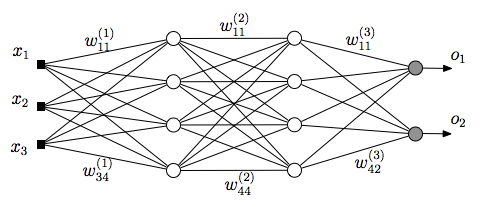
\includegraphics[scale=0.5]{img/MLP}
    \caption{Paveikslėlio pavyzdys}
    \label{img:mlp}
\end{figure}

\end{document}
